% !TEX root = ../thesis.tex

\chapter{Analytical part} \label{sec:analytical}

\section{Introduction to the issue} \label{sec:description}
Each e-commerce project solves how to predict behavior of their consumers or visitors.
In that complex prediction is usually used statistical methods like a moving average and linear regression to get an idea of consumers behavior.
Basically we need to calculate conversion rate, bounce rate, income value per order and per a customer.
Problem of that values is their non-predictable state by ordinary methods.
Based on Time series analysis we are able to predict future income but with unsatisfactory aberration.
Better results is produced by trigonometric and polynomial functions as a prediction model.
However on these methods psychology and sociology aspects are not applicable.
There are many statistical methods usable for income prediction, but in many cases the reality
of the products' life have to be really different, and these non-relevant data will make managerial decisions more
difficult to reflect prediction in company business model and cash flow.
So let us to create better complex models solution to predict company income with minimal aberration.
The best approach is to create business plans with that modeling before, so we can minimize the risk of our business.
Two phenomena of particular interest in assessing modelling options are the decoy effect~\ref{subsec:decoy} and vendor lock-in~\ref{subsec:lock-in} principles.
As is written in Models of Consumer Behaviour~\cite{patel}, this modelling is especially used when the new brand or product is established.
Let us to learn e-commerce business used them on daily basis and break the obstacle like a research price for that studies.\\
\\
\textbf{Decoy effect} \label{subsec:decoy}\\
The Decoy Effect or the Asymmetric Dominance Effect is a cognitive bias in which consumers will tend to have a specific
change in preferences between two vendor options when also presented with a third option that is asymmetrically dominated.
Simply put when there is a third strategically important choice, like the decoy, then the consumer is more likely to choose the more expensive of the other two options.
An option is asymmetrically dominated when it is inferior in all respects to one option.
However, in comparison to the other option, it is inferior in some respects and superior in others.
In other words, it is completely dominated by one option and only partially dominated by the other.
When the asymmetrically dominated option is present, a higher percentage of consumers will prefer the dominating
option than when the asymmetrically dominated option is absent.
The asymmetrically dominated option is therefore a decoy serving to increase preference for the dominating option.\\
\\
\textbf{Lock-in} \label{subsec:lock-in}\\
Proprietary lock-in, or consumer lock, makes the consumer dependent on the products and services of a particular
entity by creating significant costs of switching to the products and services of others.
This can be achieved, for example, by the use of non-standardized patented product components.
Locking, which creates barriers to market entry, can be avoided by antitrust measures.
Proprietary locking is for example blocking mobile phones for only one of the operators or DRM.
\\
\section{Mathematical background and models} \label{sec:introduction}
Overview of mathematical equations and approaches used to our prediction in context of Marketing approaches usually used to predict consumer behavior.\\
\\
\textbf{Simple Dynamic Models} \label{subsec:simpleDynamicModels}\\
One of the simplest models that have been considered for human behavior modeling are dynamic single prices~\cite{pantland}:

\begin{equation} \label{eq:1}
X_k = f(X_k, t) + \xi(t),
\end{equation}
\\
where the function $f$ is dynamic evolution of vector $X_k$ at time $k$. $\xi$ is white noise process having known spectral density matrix.
Then we can define an observation process like~\cite{pantland}:

\begin{equation} \label{eq:2}
Y_k = h(X_k, t) + \eta(t),
\end{equation}
\\
where the sensor observation $Y$ is a function of $h$ of the state vector and time. $\eta$ is white noise process having known spectral density matrix.\\
\\
Using Kalman's results we can than found the optimal linear estimate as you can see in equation~\ref{eq:3}.\\
\\
\textbf{Multiple Dynamic Models} \label{subsec:multipleDynamicModels}\\
The consumer behavior is usually not as simple as a single dynamic model.
For complex model of human behavior we can use some alternatives.
In many cases we have to use different models for each person's dynamic response~\cite{wilsky}.
Then we can test each instance of response to predict a person's state.
From that we can establish multiple model approach to predict future values of state variables.
In these situations is Kalman's filter calculation very usefully for realtime application because of it's sufficiently small costs of resources.
This approach breaks the person's overall behavior down into several prototypical behaviors~\cite{pantland}.
Mathematically, this is accomplished by setting up a set of states $S$, each associated with a Kalman's filter and a particular dynamic model.\\
\\
\textbf{A linear ODE model} \label{subsec:ode}\\
In this model the strength of flux between brands or products are determined by perceived brand quality,
based upon binary comparisons.
The simplest response to such comparisons is an attempt by customers to minimize the expected regret resulting
from any choice, which is what is assumed here.
It has previously been shown that the choice rule recognizes the attribute-wise proximity of an alternative
to other brands, and it is therefore appropriate for preference change to be modelled on the pair-wise ranking
of brands in each quality, the simplest perhaps being to assign a positive score to a brand for each successful comparison.
Thus, customers attempt to minimize their anticipated regret by opting – on any particular quality – for the safe bet.
More sophisticated customer behavior, capable of not only ranking brands but discriminating according to the size of proximity gap
requires more complex modelling, but may be justified since it appears that subjective attribute valuations at least are nonlinear, reference-point-dependent functions.\\
\\
\\
\\
\\
\\
\textbf{Discrete-time model} \label{subsec:discrete}\\
Discrete models or difference equations \footnote{Difference equations can be viewed either as a discrete analogue of differential equations, or independently.
They are used for approximation of differential operators, for solving mathematical problems with recurrences, for building various discrete
models, etc.} are used to describe biological events or whole systems for which is natural to regret time at fixed discrete intervals~\cite{pantland}:

\begin{equation} \label{eq:3}
\hat{X}_{k}^{(i)} = X_{k}^{*(i)} + K_k^{(i)}(Y_k - h^{(i)}(X_{k}^{*(i)},t)),
\end{equation}
\\
where the superscript $(i)$ denotes the $i$th Kalman's filter.
As input $K_k$ Kalman's gain matrix is used for time step $k$.
Then sensor observator $Y$ from equation~\ref{eq:2} is used in combination with $X_{k}^{*}$ as a state prediction matrix.
The measurement innovations process for the $i$th model.\\
\\
The $i$th measurement innovations process is, intuitively, the part of the observation data that is unexplained by the $i$th model.
The model that explains the largest portion of the observations is, of course, the model most likely to be correct.\\

\subsection{Modeling and Prediction of Human Behavior} \label{subsec:prediction}
Based on equation~\ref{eq:3},\ we can continue to find optimal linear estimate $X_k$ using th Kalman's filter~\cite{pantland}: \footnote{In statistics
and control theory, Kalman filtering, also known as linear quadratic estimation (LQE), is an algorithm that
uses a series of measurements observed over time, containing statistical noise and other inaccuracies, and produces
estimates of unknown variables that tend to be more accurate than those based on a single measurement alone, by estimating
a joint probability distribution over the variables for each timeframe.
The filter is named after Rudolf E. Kálmán, one of the primary developers of its theory.}

\begin{equation} \label{eq:5}
X = X_{k}^{*} + K_x(Y_k - h(X_{k}^{*},t)),
\end{equation}
\\
provided that the Kalman gain matrix $K_k$ is chosen correctly~\cite{kalman}.
This method iterates for each step $k$ and the filter algorithm use a state prediction at each time step $k$,
the filter algorithm uses a state prediction $X$, an error covariance matrix prediction $P_k^*$,
and a sensor measurement $Y_k$ to determine an optimal linear state estimate $X$.
If we want to predict human's future state whe can use this mechanism with larger time steps.
This mechanism is used e.g. in a car, such a prediction capability can allow us to maintain synchrony with the driver.
In experience of Alex Pentland work \footnote{MIT's Human Dynamics Laboratory and the MIT Media Lab Entrepreneurship
Program, co-leads the World Economic Forum Big Data and Personal Data initiatives, and is a founding member
of the Advisory Boards for Nissan, Motorola Mobility, Telefonica, and a variety of start-up firms.}, this type of prediction
is useful only for short time periods, for instance, in the case of quick hand motions for up to one-tenth of a second.
Especially $f$, $h$ are linear functions and $\xi$, $\eta$ are gaussian.
These functions are commonly extended to "well-behaved" nonlinear problems by approximating the nonlinear system by linear functions
using a local Taylor expansion \footnote{Taylor series is a representation of a function as an infinite sum of terms that are calculated from
the values of the function's derivatives at a single point.}.

\subsection{Specification in customer behavior} \label{subsec:specification}
Customer products such as shampoo or tomato sauce are designed to appeal to customers, encouraging them to buy those products.
It depends on the industry section but all of that designs trying to focus to customer's subconscious.
However, buying behavior is not only a function of the product.
In many cases is the connection of many other functions like a social environment of other customers, the competing
products in the marketplace, brand marketing strategy, seller trust and professionalism and so on.
In order to design the best product, it is necessary to understand not just the physics and chemistry of the product,
but also the psychology of customers and the sociology of customer groups or networks\cite{patel}.

From that paragraphs is seen that the general customer behavior model has many input variables to represent many kinds
of situations to be successfully in future prediction.
Good model in store industry have to be able to learn from actual customer's behavior for each seller and learn
from these datasets in a macroscopic, averaged way.
Alternatively, one can look at individual customers, and their buying behavior, and try to derive observable large scale effects.
Ideally it can be predicted behavior for each customer and from these results create a global results for each store or industry.\\
\\
\textbf{Loyalty} \label{subsec:loyalty}\\
Loyalty is the tendency for some customers to use the same products or brands again.
This behavior we can describe with a systems of ordinary differential equations.
The stronger the loyalty, the slower the changes in numbers of people buying particular products.
For discrete-time models, the degree of loyalty corresponds to the size of diagonal elements in a transition matrix.
In the modelling we have to calculate with the no loyalty model too.
In some industries like a supermarkets, peoples buy from other reason, so some of our input variables in modelling should be
detection of loyalty in out industry.
Next aspect of loyalty would be a memory effect, to represent people returning to products they had previously used,
after trying something new they then did not like.
This could be taken into account perhaps by using recurrence relations or differential equations of higher than first order or even employing
delay-differential equations.\\
\\
\textbf{Sociology} \label{subsec:sociology}\\
Mean sociology in this context as how peoples buying are influenced each other.
With some kind of trends to buy the same brands or products.
There is an option from lock-in~\ref{subsec:lock-in}, with one product dominating the market.
This option is very hard to relevant test, because of the data of huge companies which dominates some kind
of industry are very hard to legally get.
Even if theirs competitors have more or less identical products.
This effect and its opposite, are easily modelled by ODE~\ref{subsec:ode} and discrete-time models.
Opposite is very important in sociology because of people wanting to be different sometimes from irrationals reasons.

\subsection{Markov Chains} \label{subsec:chain}
A Markov chain is a process that occurs in a series of time-steps in each of which a random choice is made
among a finite (or also enumerable) number of states since both the index set and the state space are discrete,
as is seen on figure~\ref{markovmodel}, then we denote by~\cite{patel}:\\
\begin{equation} \label{eq:6}
\begin{array}{l@{}l}
	p_{ij}=P[X_{n+1}=j|X_n=i],
\end{array}
\end{equation}\\
where $p_{ij}$ is the probability of moving from state $i$ to state $j$, then the transition probability is represented by a matrix.\\
For homogeneous chains, these probabilities do not depend on $n$, i.e., they are stationary.
Then, the initial distribution, together with the transition matrix $P$, determines the probability distribution for any state at all future times.\\
\begin{figure}[h!]
	\begin{center}
		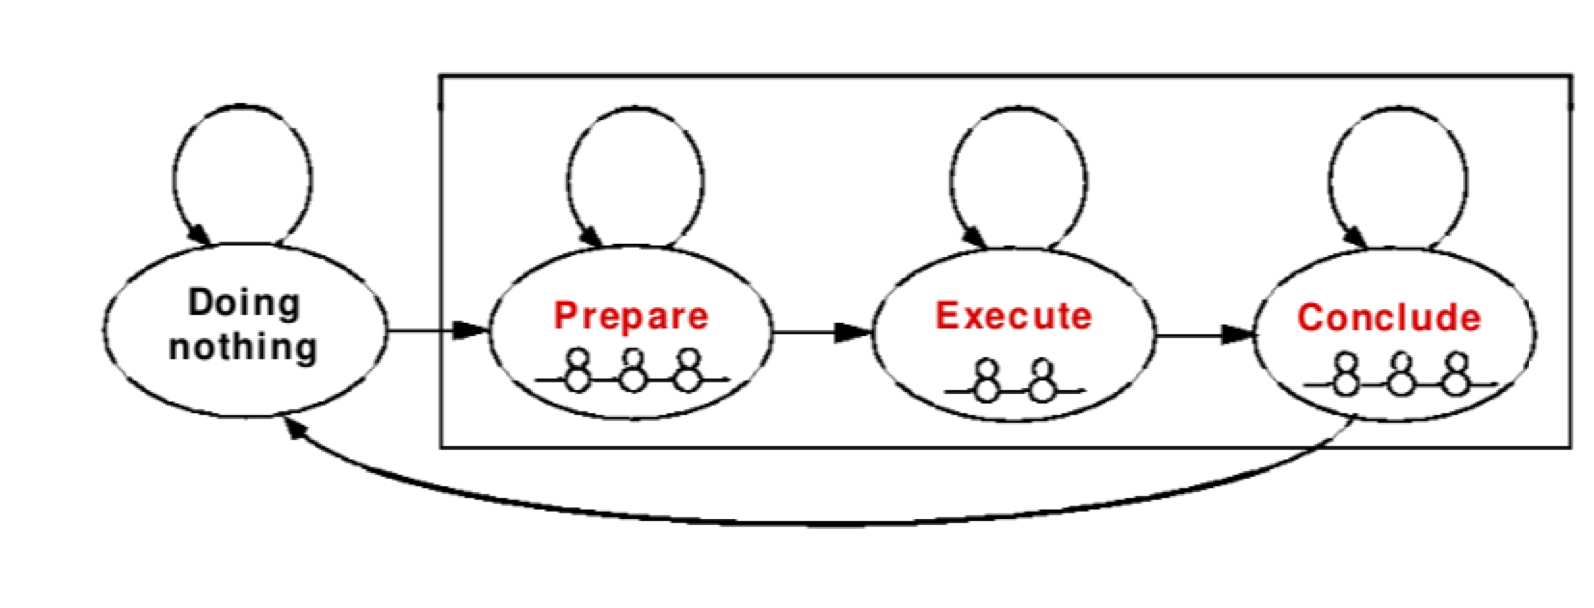
\includegraphics[width=140mm]{markov_model.png}
	\end{center}
	\caption{Basic schema of Markov model in human decision~\cite{patel}}
	\label{markovmodel}
\end{figure}
\\
\textbf{A Markov model with social influences} \label{subsec:markov}\\
This model is based on Markov chains (Markov chain description), better than the time continues differential
equations which are especially used.
To use that model approach we first have to develop the possibility of a decoy effect.
Then we introduce sociology and obtain results for lock-in analogous.
These Markov models display both important similarities to and differences from the previous models, and may be simpler to work with.
The last but not the least pros of that models is very good graphical representation.\\
\\
\textbf{An Experiment Using Markov Dynamic Models} \label{subsec:markov_dynamic}\\
Shopping is natural-feeling and familiar type of human behavior that exhibits complex patterns that last from several
seconds to many days.
These characteristics make shopping little nearly ideal experimental for modeling human behaviors.
In the case of shopping, the macroscopic actions are events like needs, choosing brands, choosing seller.
The internal states are the individual steps that make up the action, and the observed variables will be changes during the shopping process
workflow in which can be customer decision changed.
The intuition is occasionally important, but this belongs to special market and marketing persons identification such
a buying shoes by a single woman in production age.\\
\\
\textbf{Modeling and Prediction of Human Behavior may consist of the following steps:}\\
\begin{enumerate}
	\item needs decision make
	\item looking across the site to find some adequate
	\item make action decision
	\item shopping workflow process in selected site
	\item make final payment
\end{enumerate}
\\
Psychology covers what, and how, aspects of the actual items on the shelves influence people to make their choices,
possibly buying something different from previously.
Advertising might be comprised into these characteristics but could also possibly be considered as part of the sociological
influences (point 1 and 2), especially if the advertising takes the form of a well known figure endorsing a product.
More specifically, the following four properties have been identified by Unilever Research~\cite{patel} as being important
and their influences were included in one or more models:

\begin{enumerate}
	\item Minimise anticipated regret.
	This refers to how just two products compare with each other as regards different qualities, which can include
	price (or affordability = 1/price).
	A customer might judge one item to be superior to another in all respects.
	The first is then a safe choice for the customer.
	\item Attribute change.
	The introduction of a new product onto the market can change the way customers, or at least some of them, view established brands.
	This might be by drawing attention to some quality which was not previously much regarded, or it might make people give different
	weightings to the (established) qualities when making their decisions.
	The former can be considered to be a special case of the latter.
	\item Outlier avoidance.
	When a number of products are in many aspects quite similar, there can be a tendency for people to avoid ‘strange’ ones, like others which
	are substantially different from the majority in price or some other respect.
	Items near the average can be favoured.
	\item Decision process change.
	A straight choice between two items might be relatively easy.
	They can be compared according to price, size etc\. and a decision made.
	With three or more, comparisons might be made between two things at a time, one could be eliminated and then the winner contrasted
	with a third.
\end{enumerate}

\subection{Networks} \label{sec:networks}
Markov chain propagation should be imagine as decision tree with a predefined states and probabilities from one state to another.
To see how such a model gives rise to the probabilities of choosing each state we need to
construct a decision tree. In forming the decision tree we have to decide which states the consumer
will choose to compare. This process should be done eg. in Hidden markov chain.
There is an equal probability of choosing each pair. We also have to decide how many comparisons the consumer
will make, that is, having chosen a final state.\\
\begin{figure}[h!]
	\begin{center}
		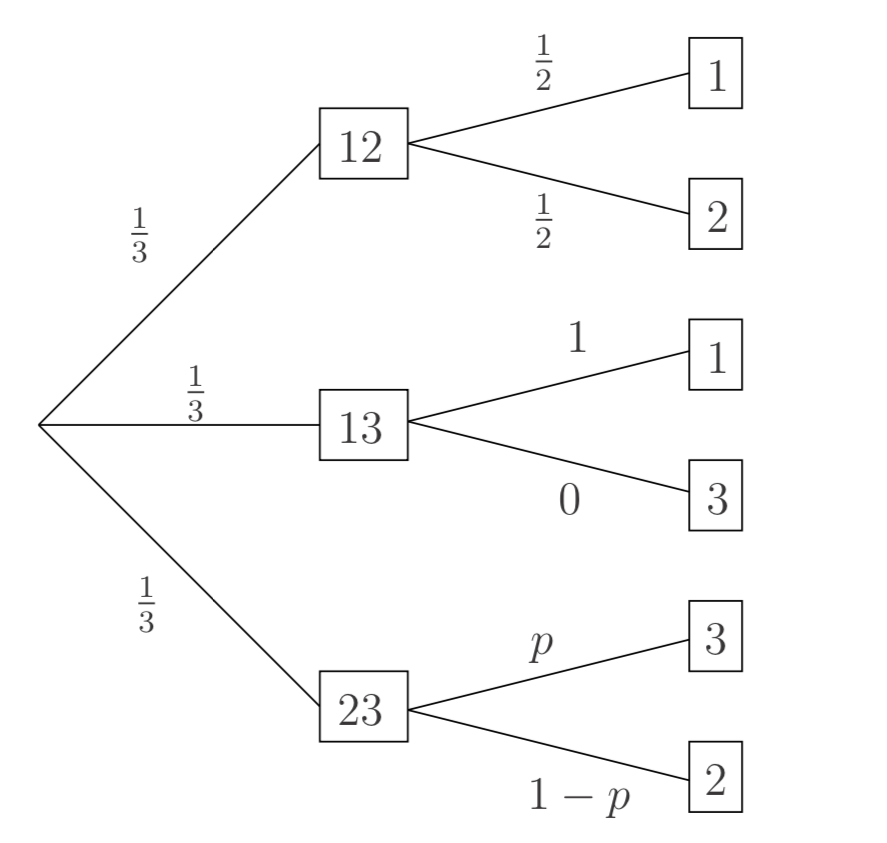
\includegraphics[width=80mm]{level1DT.png}
	\end{center}
	\caption{Schema of decision tree function~\cite{patel}}
	\label{DT1}
\end{figure}\\
The simplest decision tree for the three states shown in Figure~\ref{DT1}, with one level of
comparison (that is, the consumer stops after comparing just two states eg. continue order or leave the store)
For better explanation look let us assume that products 1 and 2 are equally attractive to the consumer, so that in the absence of
product 3 each would have a probability of selection of 1/2.
We can then see what the introduction of product 3 does to this balance of probabilities, and in particular whether there is a decoy effect (See section ~\ref{subsec:decoy}),
that is, since product 1 dominates product 3, the introduction of product 3 might mean that more people will choose to buy product 1 (since product 1 will win in any comparison between the two).
In this scenario product 3 acts as a decoy, channelling consumers to product 1.
Let us assume that the probability of choosing product 3 over product 2 in a comparison is $p$.\\
The probability of reaching any leaf in the decision tree is simply the product of the probabilities of
taking each branch required to get there.
Thus, after introducing product 3 the probabilities of choosing each product are~\cite{patel}:\\

\begin{equation} \label{eq:12}
\begin{array}{l@{}l}
	p_1 = \frac{1}{3}*\frac{1}{2}+\frac{1}{3}*1 = \frac{1}{2} \\
	p_2 = \frac{1}{3}*\frac{1}{2}+\frac{1}{3}*(1-p) = \frac{1}{2} - \frac{p}{3} \\
	p_3 = \frac{1}{3}*0+\frac{1}{3}*p = \frac{p}{3},
\end{array}
\end{equation}\\
where $p_1,p_2,p_3$ are probabilities for each state and $p$ is the probability of choose product 3 over product 2.\\
\\
\subsection{Viterbi algorithm} \label{subsec:viterbi}
The Viterbi algorithm is a dynamic programming algorithm for finding the most likely sequence of hidden
states called the Viterbi path that results in a sequence of observed events, especially in the
context of Markov information sources and hidden Markov models (HMM) as it sens on figure~\ref{viterbi-schema}.
\begin{figure}[h!]
	\begin{center}
		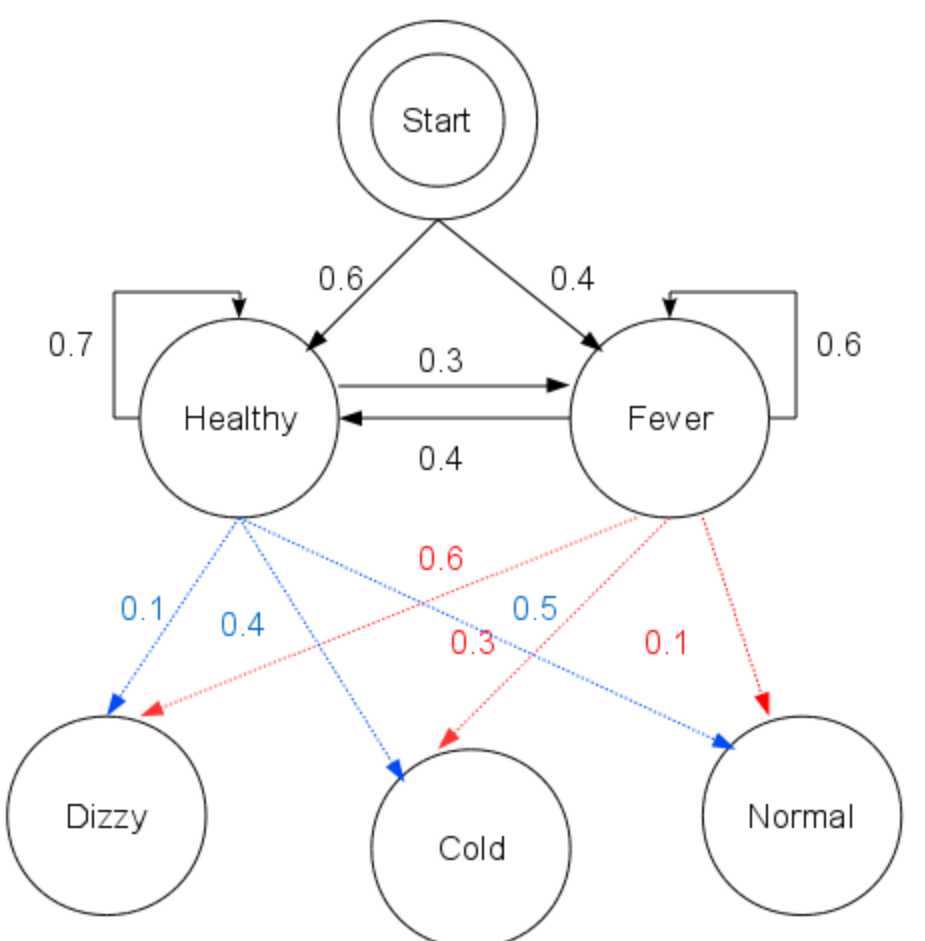
\includegraphics[width=80mm]{viterbi_graph.png}
	\end{center}
	\caption{Viterbi algorithm schema example~\cite{viterbi}}
	\label{viterbi-schema}
\end{figure}\\
The algorithm has found universal application in decoding the convolutional codes used in
both CDMA and GSM digital cellular, dial-up modems, satellite, deep-space communications, and 802.11 wireless LANs.
It is now also commonly used in speech recognition, speech synthesis, keyword spotting, computational
linguistics, and bioinformatics.
For example, in speech-to-text (speech recognition), the acoustic signal is treated as the observed sequence of events,
and a string of text is considered to be the "hidden cause" of the acoustic signal.
The Viterbi algorithm finds the most likely string of text given the acoustic signal.\\
Here you can see Viterbi algoritm implementation in Python language~\cite{DBLP:journals/corr/abs-cs-0504020}: \\
\begin{python}
# probability == p. Tm: the transition matrix. Em: the emission matrix.
function viterbi(O, S, Π, Tm, Em): best_path
  # To hold p. of each state given each observation.
  trellis ← matrix(length(S), length(O))
  # Determine each hidden state's p. at time 0…
  for s in range(length(S)):
    trellis[s, 0] ← Π[s] * Em[s, O[0]]
  # and afterwards, assuming each state's most likely prior state, k.
  for o in range(1, length(O)):
    for s in range(length(S)):
      k ← argmax(k in trellis[k, o-1] * Tm[k, s] * Em[s, o])
      trellis[s, o] ← trellis[k, o-1] * Tm[k, s] * Em[s, o]
  best_path ← list()
  # Backtrack from last observation.
  for o in range(-1, -(length(O)+1), -1):
    # Most likely state at o
    k ← argmax(k in trellis[k, o])
    # is noted for return.
    best_path.insert(0, S[k])
  return best_path
\end{python}\\

\subsection{Predicted effects} \label{subsec:predicted}
\begin{enumerate}
	\item How a decoy product might influence the market.
	The appearance of a third product might remarkably change the market shares of two others, while getting minimal sales itself.
	This effect is one of the most complex biases in customer choice, and has been observed in product classes from chocolate bars
	to electronics to beer.
	The decoy effect illustrates the importance of customer psychology, to understanding how customers recognize products,
	and how customers see quality side to buy the product.

	\item The dynamics of market share is  how sales of products can change during the time.
	For example, even if two products are really equal in all relevant aspects, then after a long time of customer activity it might be that
	each product takes 50\% market share (preserving the symmetry), or one product takes nearly 100\% market share (breaking the symmetry),
	or that there is no steady state, with market dominance alternating between the two brands.
	The second of these three cases is called lock-in, corresponding to one brand obtaining a virtual monopoly,
	which is almost impossible to break.
	From that reason is not legally to create a monopole in some industries and for human purchase behavior is not
	good to calculate with monopole approach.

	\item How a new product will fare, given its quality profile compared with existing brands.
	This question is complementary to that of the decoy, asking what market share a new product will gain rather than how it will
	affect the market shares of existing products.

	\item A choice overload: when there are just too many possible options for potential customers to pick from, and many
	will search the sites without making a purchase.
\end{enumerate}

\subsection{Minimise anticipated regret} \label{subsec:regret}
This modelling property was taken to lead to simple comparisons along the lines of with regard to quality $k$,
is product $i$ better than product $j$?
If the answer to all relevant questions, $k = 1, . . . , nq$, if $nq$ is the number of qualities, is no, then a customer
will not change from $j$ to $i$.
The more times the answer is yes, the faster such a change is likely to happen.
This can be represented by taking the flow-rate constants to be of the form (todo equation)

\section{Customer preferences and decision process} \label{sec:customer_preferences}
Consider a customer whose preference is shared out amongst all the available brands in a market where there are
no empty or zero brands, so that the total of all brands preference shares is 1 (100\%).
The proportion of customer preference held by brand $X$ at time $t$ is denoted by $X(t)$.
For example, if the preference share of brand $A$ is plotted against brand $B$ in a market where only two brands exists,
the point must be somewhere along the straight line $B(t) = 1, A(t)$.
Of interest is the case when a third brand is added, possibly as a decoy.
The additional brand means that the preference distribution changes from being a straight line in the two-dimensional plane $(A, B)$,
to a plane in three-dimensional space $(A,B,C)$.\\
\\
\textbf{Customer decision process} \label{sec:cus_decision}\\
Described in~\cite{patel} show that the standard Logit model~\ref{subsec:logit} for customer choice assumes that
the probability, $p_i$, with which a customer buys a given product $i$ from a range of products $<1, n>$ depends on
the value which customer internally assigned to that product and his price.
This dependence is taken to be of exponential form.
Assuming that guaranteeing that all probabilities are positive)
\\
\begin{equation} \label{eq:7}
p_i = C\exp(V_i - sP_i),
\end{equation}
\\
where $s$ is a measure of the relative importance of price to the customer, and $C$ is a normalisation constant set to be results always positive. $V_i$ is subjective value
attached to product by a customer with dependency on price of the product $P_i$.~\cite{patel}.
\\
\begin{equation} \label{eq:8}
\sum_{i=1}^n p_i = 1
\end{equation}
\\
The value $V_i$ is then taken to reflect the influence on the customer of the quality of the product,$Q_i$,
the increased likelihood of the customer buying the same brand as he bought previously (the loyalty effect),
and the peoples who have an influence on a customer (neighbours).
Each of these dependencies are taken to be linear, giving~\cite{patel}:
\\
\begin{equation} \label{eq:9}
V_i = aQ_i + lI_i + hN_i,
\end{equation}
\\
where $I_i$ is an indicator function which is unity if the customer a previously bought product i and zero otherwise,
$N_i$ is the number of neighbours who bought product $i$, and $a, l$ and $h$ are constants measuring the relative strength
of each effect.
In such a model the products are all treated independently.
Only coupling between the probabilities occurs through the normalisation constant $C$.
Product $I$ will depend not only on the value and price of that product, $V_i$ and $P_i$, but on the value and prices of all products.
The goal of this section is to formulate a model for this probability which is based on binary comparisons, that is,
on comparisons of two products at a time.\\
\subsection{Logit analysis in marketing} \label{subsec:logit}
Logit analysis is a statistical technique used by marketers to assess the scope of customer acceptance of a product, particularly a new product.
It attempts to determine the intensity or magnitude of customers' purchase intentions and translates that into a measure of actual buying behavior.
Logit analysis assumes that an unmet need in the marketplace has already been detected, and that the product has been designed to meet that need.
The purpose of logit analysis is to quantify the potential sales of that product.
It takes survey data on consumers purchase intentions and converts it into actual purchase probabilities.
Logit analysis defines the functional relationship between stated purchase intentions and preferences, and the actual probability of purchase.
A preference regression is performed on the survey data.
This is then modified with actual historical observations of purchase behavior.
The resultant functional relationship defines purchase probability.

\subsection{Brand or product changing} \label{subsec:brand}
We can mathematically express the process of decision to switch from one brand to another one.
Consider a linear flux $\alpha_{xy}$ of preferences moving to brand $X$ from brand $Y$.
All fluxes have to be strictly positive.
It's in improper to consider negative flux, so really excluded is only zero value.
Flux is the proportion of customer preference to switch to other brand or product from previous one.
\begin{figure}[h!]
	\begin{center}
		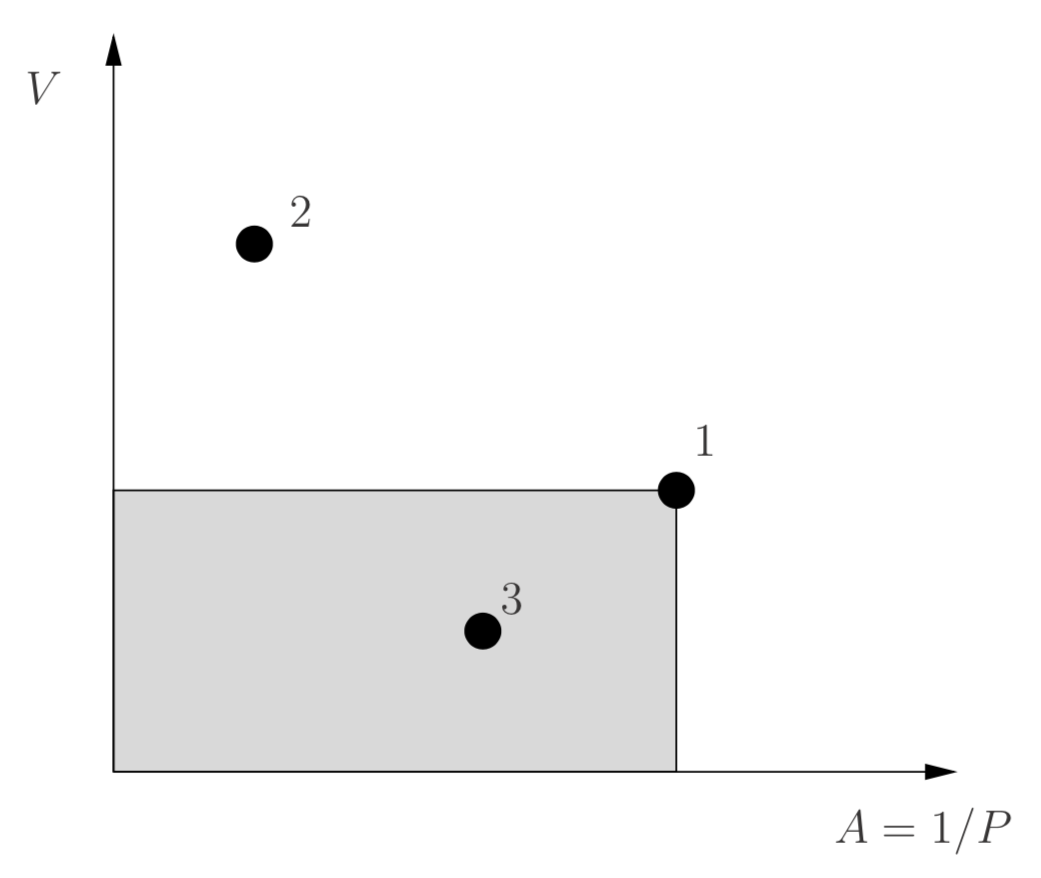
\includegraphics[width=80mm]{affordability.png}
	\end{center}
	\caption{Products in the affordability-value plane.
	The shaded region is the region of products dominated by product 1.}
	\label{Affordability of products~\cite{pantland}}
\end{figure}
\\
\section{A particle-dynamics model} \label{sec:dynamic}
The basic idea from Models of Consumer Behaviour~\cite{patel} is to build a model based on a physical analogy, between the customers buying behavior
and particle-particle dynamics.
Lets us assume customers to be particles moving in quality space.
\begin{figure}[h!]
	\begin{center}
		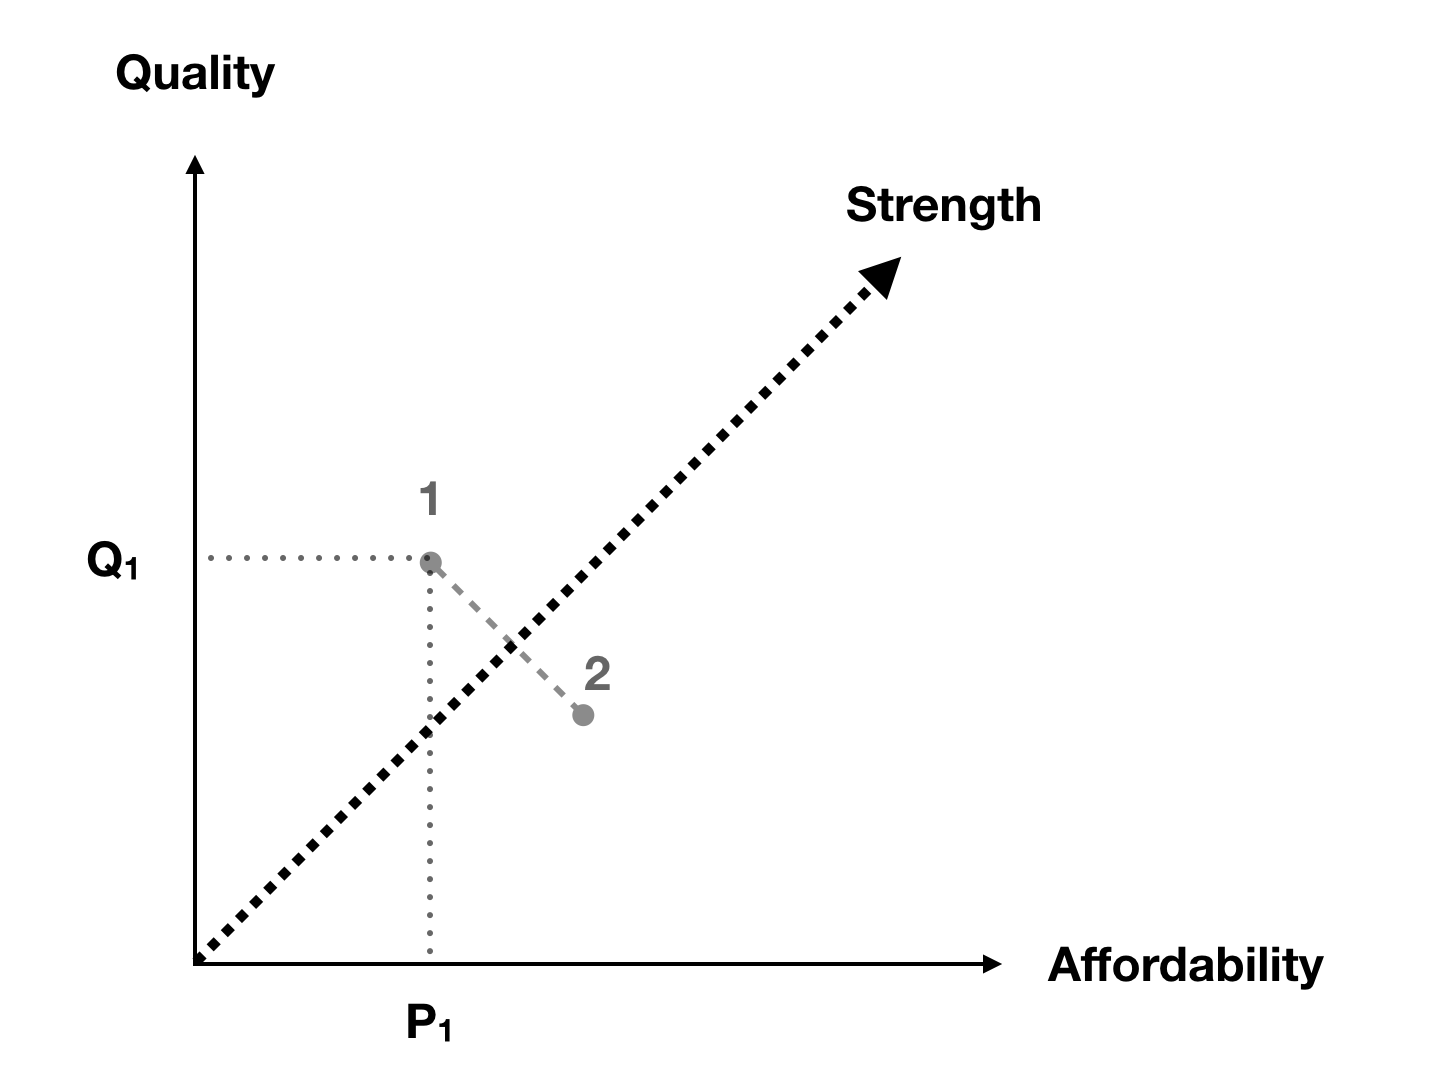
\includegraphics[width=80mm]{strength.png}
	\end{center}
	\caption{Product space with two products}
	\label{Strength of products~\cite{patel}}
\end{figure}
\\
The products are considered as sources of strength potentials, the details of the potentials depending on the products’ characteristics.
The psychology of people will be regarded as the influence of the potential on the mass of the particles.
This will depend on the customer but also on the characteristics of each product, weighted by coefficients of choice.
The sociology of individuals can be considered as a form of particle-particle interaction.
Following what has gone before, the product space is defined by just two characteristics for each product $i$ with affordability $P_i$ and quality $Q_i$.
We can define the ‘strength’ \footnote{ thw power if the product or service to be attractive for customer} of a product as the distance
of the product from the origin in product space as~\cite{pantland}:
\\
\begin{equation} \label{eq:10}
U_i = \frac{(P_i + Q_i)}{2}.
\end{equation}
\\
All the products with $P_i + Q_i = constant$ will have the same strength.

\subsection{Dynamics of market share} \label{subsec:marketshare}
Market shares don't unusually depend on their qualitative behavior, on the coefficients $\alpha_{ij}$ and the values
of $\alpha_{ij}$ grow up as fast as their tend towards stability values.
In the situation  that $\alpha_{ij} \geq 0$ and $\alpha_{ij} + \alpha_{ji} > 0$ for $i \neq j$ the linear system looks like~\cite{patel}:
\\
\begin{equation} \label{eq:17}
\frac{dX_i}{dt} = \sum_ja_{ij}X_j,
\end{equation}
\\
where $a_{ij} = \alpha_{ij}$ for $i \neq j$ and $a_{ii} - \sum_{i \neq j}\alpha_{ji}$ turns out to have semi-definite
coefficient matrix.

\section{Regression} \label{sec:regression}
As a baseline for our model will be used linear and linear and polynomial fitting.
Lets create two models to predict future income.\\
\subsection{Linear regression} \label{sec:linear}
As it saw at Linear regression~\cite{linear} linear regression attempts to model the relationship between two variables by fitting a linear equation to observed data.
One variable is considered to be an explanatory variable, and the other is considered to be a dependent variable.
For example, we want to relate the weights of individuals to their heights using a linear regression model.
Before attempting to fit a linear model to observed data, we should first determine if exist a relationship between the variables of interest.
This does not necessarily mean that one variable causes the other, but that there is some significant association between them.
To determine the strength of relationship a scatterplot can be a helpful tool.
If there appears to be no association between the proposed explanatory and dependent variables, then fitting a linear regression
model to the data probably will not provide a useful model.
A valuable numerical measure of association between two variables is the correlation coefficient.
That is a value from $<-1, 1>$ range indicates the strength of the association of the observed data for the two variables.\\
A linear regression line has an equation of the form $Y = a + bX$, where $X$ is the explanatory variable and $Y$ is the dependent variable.
The slope of the line is $b$, and $a$ is the intercept.

\subsection{Polynomial regression} \label{sec:poly}
Polynomial models are a great tool for determining which input factors drive responses and in what direction~\cite{poly}.
These are also the most common models used for analysis of designed experiments.
A quadratic (second-order) polynomial model for two explanatory variables has the form of the equation below.
The polynomial models can be used in those situations where the relationship between study and explanatory variables is curvilinear.
Sometimes a nonlinear relationship in a small range of explanatory variable can also be modelled by polynomials.
The order of the polynomial model is kept as low as possible.
Some transformations can be used to keep the model to be of the first order.
If this is not satisfactory, then the second-order polynomial is tried.
A good strategy should be used to choose the order of an approximate polynomial.
One possible approach is to successively fit the models in increasing order and test the significance of regression coefficients at each step of model fitting.
Another approach is to fit the appropriate highest order model and then delete terms one at a time starting with the highest order.
This is continued until the highest order remaining term has a significant statistic.
This is called a backward elimination procedure.
The forward selection and backward elimination procedures do not necessarily lead to the same model.
The first and second-order polynomials are mostly used in practice.
Keep the order increasing until test for the highest order term is nonsignificant.
This is called a forward selection procedure.
Arbitrary fitting of higher-order polynomials can be a serious abuse of regression analysis.
A model which is consistent with the knowledge of data and its environment should be taken into account.
It is always possible for a polynomial of order to pass
through n points so that a polynomial of sufficiently high degree can always be found that provides
a good fit to the data.
Such models neither enhance the understanding of the unknown function nor be a good predictor.
